\chapter{Метод построения оптимального порядка перезагрузки}\label{method}
В данной главе будут рассмотрены методы построения оптимального порядка перезагрузки реактора.
Будет описан метод поиска порядка в графовом представлении ТА-модели реактора, а также исследованы алгоритмы поиска кратчайшего пути в графе.

\section{Поиск оптимального порядка в ТА-модели реактора}
Описанная в разделе~\ref{TA-model} модель реактора обладает следующими свойствами:
\begin{itemize}
 \item [-] состояние ТА-модели $q_0$ является моделью состояния реактора к началу планово-профилактического ремонта;
 \item [-] состояния ТА-модели из множества $F$ являются искомыми состояниями, в которых планово-профилактический ремонт будет завершен;
 \item [-] входное слово для ТА-модели является последовательно выполняемыми действиями над реактором, которые приводят его в новое состояние.
\end{itemize}
Таким образом, задача построения порядка проведения планово-профилактического ремонта реактора сводится к поиску входных слов конечного автомата, которые приводя его в конечное состояние.

Описанный в разделе \ref{automata-theory} метод описания детерминированных конечных автоматов в виде диаграммы переходов представляет собой ориентированный граф.
Вершинами графа являются состояния автомата, а ребрами графа --- символы входного алфавита автомата. 
Тогда становится возможным произвести поиск по графу из вершины $q_0$ в вершины из множества $F$, используя алгоритмы поиска пути в графе (будут рассмотрены далее).

Каждое действие, производимое над реактором имеет различные трудо- и энергозатраты, следовательно для построения оптимального порядка перезагрузки требуется учитывать эти затраты в модели.
Установим в соответствие каждому входному символу КДА коэффициент затрат и введем его в ТА-модель.
Для этого каждому ребру графа поставим в соответствие коэффициент затрат, т.е. сделаем граф взвешенным.
Тогда оптимальным порядком проведения планово-профилактического ремонта будет являться такая последовательность операций, которое приводит ТА-модель реактора из начального в конечное состояние с минимальной суммой энергозатрат.

\section{Алгоритмы поиска пути в графе}

Задача о кратчайшем пути --- задача поиска самого короткого пути (цепи) между двумя точками (вершинами) на графе, в которой минимизируется сумма весов ребер, составляющих путь.
Кратчайшая (простая) цепь часто называется геодезической. \cite{graph-harry}
Задача о кратчайшем пути является одной из важнейших классических задач теории графов. 
Сегодня известно множество алгоритмов для ее решения.
У данной задачи существуют и другие названия: задача о минимальном пути или, в устаревшем варианте, задача о дилижансе.

Задача поиска кратчайшего пути на графе может быть определена для неориентированного, ориентированного или смешанного графа. 
Далее будет рассмотрена постановка задачи в самом простом виде для неориентированного графа. 
Для смешанного и ориентированного графа дополнительно должны учитываться направления ребер.

Граф представляет собой совокупность непустого множества вершин и ребер (наборов пар вершин). 
Две вершины на графе смежны, если они соединяются общим ребром. 
Путь в неориентированном графе представляет собой последовательность вершин $P = (v_1, v_2, \dots, v_n) \in V\times V \times \dots \times V$, таких что, $v_i$ смежна с $v_{i+1}$ для $1\leqslant i < n$.
Такой путь $P$ называется путем длиной $n$ из вершины $v_1$ в $v_n$ ($i$ указывает на номер вершины пути и не имеет никакого отношения к нумерации вершин на графе).

Пусть $e_{i, j}$ --- ребро соединяющее две вершины: $v_i$ и $v_j$. 
Дана весовая функция $f: E \rightarrow \mathbb{R}$, которая отображает ребра на их веса, значения которых выражаются действительными числами, и неориентированный граф $G$. 
Тогда кратчайшим путем из вершины $v$ в вершину $v'$ будет называться путь $P = ( v_1, v_2, \ldots, v_n )$ (где $v_1 = v$ и $v_n = v'$), который имеет минимальное значение суммы $\sum_{i =1}^{n-1} f(e_{i, i+1})$. 
Если все ребра в графе имеют единичный вес, то задача сводится к определению наименьшего количества обходимых ребер. \cite{graph-evstigneev}

Существуют различные постановки задачи о кратчайшем пути:
\begin{itemize}
\item [-] Задача о кратчайшем пути в заданный пункт назначения. 
Требуется найти кратчайший путь в заданную вершину назначения $t$, который начинается в каждой из вершин графа (кроме $t$). 
Поменяв направление каждого принадлежащего графу ребра, эту задачу можно свести к задаче о единой исходной вершине (в которой осуществляется поиск кратчайшего пути из заданной вершины во все остальные).
\item [-] Задача о кратчайшем пути между заданной парой вершин. 
Требуется найти кратчайший путь из заданной вершины $u$ в заданную вершину $v$.
\item [-] Задача о кратчайшем пути между всеми парами вершин. 
Требуется найти кратчайший путь из каждой вершины $u$ в каждую вершину $v$. 
Эту задачу тоже можно решить с помощью алгоритма, предназначенного для решения задачи об одной исходной вершине, однако обычно она решается быстрее.
\end{itemize}

В различных постановках задачи, роль длины ребра могут играть не только сами длины, но и время, стоимость, расходы, объем затрачиваемых ресурсов (материальных, финансовых, топливно-энергетических и т. п.) или другие характеристики, связанные с прохождением каждого ребра. 
Таким образом, задача находит практическое применение в большом количестве областей (информатика, экономика, география и др.).

В связи с тем, что существует множество различных постановок данной задачи, есть наиболее популярные алгоритмы для решения задачи поиска кратчайшего пути на графе:
\begin{itemize}
 \item [-] Алгоритм Дейкстры находит кратчайший путь от одной из вершин графа до всех остальных. 
 Алгоритм работает только для графов без рёбер отрицательного веса.
 \item [-] Алгоритм Беллмана -- Форда находит кратчайшие пути от одной вершины графа до всех остальных во взвешенном графе. 
 Вес ребер может быть отрицательным.
 \item [-] Алгоритм поиска A* находит маршрут с наименьшей стоимостью от одной вершины (начальной) к другой (целевой, конечной), используя алгоритм поиска по первому наилучшему совпадению на графе.
 \item [-] Алгоритм Флойда --- Уоршелла находит кратчайшие пути между всеми вершинами взвешенного ориентированного графа.
 \item [-] Алгоритм Джонсона находит кратчайшие пути между всеми парами вершин взвешенного ориентированного графа.
 \item [-] Алгоритм Ли (волновой алгоритм) основан на методе поиска в ширину. 
 Находит путь между вершинами $s$ и $t$ графа ($s$ не совпадает с $t$), содержащий минимальное количество промежуточных вершин (ребер). 
 Основное применение --- трассировки электрических соединений на кристаллах микросхем и на печатных платах. 
 Так же используется для поиска кратчайшего расстояния на карте в стратегических играх.
 \item [-] Поиск кратчайшего пути на основе алгоритма Килдала.
\end{itemize}

Далее рассмотрим подробно алгоритм Дейкстры, алгоритм А* и волновой алгоритм. 

\subsection{Алгоритм Дейкстры}

Алгоритм Дейкстры --- алгоритм на графах, изобретённый нидерландским ученым Эдсгером Дейкстрой в 1959 году. Алгоритм Дейкстры решает задачу о кратчайших путях из одной вершины для взвешенного ориентированного графа $G = (V, E)$ с исходной вершиной $s$, в котором веса всех рёбер неотрицательны ($\omega(u, v) \geqslant 0$ для всех $(u, v) \in E$).

\textbf{Формальное объяснение}.
В процессе работы алгоритма Дейкстры поддерживается множество $S\subseteq V$, состоящее из вершин $v$, для которых $\delta(s, v)$ уже найдено. 
Алгоритм выбирает вершину $u \in V\\S$ с наименьшим $d[u]$, добавляет $u$ к множеству $S$ и производит релаксацию всех рёбер, выходящих из $u$, после чего цикл повторяется. 
Вершины, не лежащие в $S$ , хранятся в очереди $Q$ с приоритетами, определяемыми значениями функции $d$. Предполагается, что граф задан с помощью списков смежных вершин.

\textbf{Не формальное объяснение}.
Каждой вершине из $V$ сопоставим метку --- минимальное известное расстояние от этой вершины до $a$. 
Алгоритм работает пошагово --- на каждом шаге он <<посещает>> одну вершину и пытается уменьшать метки. 
Работа алгоритма завершается, когда все вершины посещены.

\textbf{Инициализация}. 
Метка самой вершины $a$ полагается равной $0$, метки остальных вершин --- бесконечности. 
Это отражает то, что расстояния от $a$ до других вершин пока неизвестны. 
Все вершины графа помечаются как непосещенные.

\textbf{Шаг алгоритма}. 
Если все вершины посещены, алгоритм завершается. 
В противном случае из еще не посещенных вершин выбирается вершина $u$, имеющая минимальную метку. 
Мы рассматриваем всевозможные маршруты, в которых $u$ является предпоследним пунктом. 
Вершины, соединенные с вершиной $u$ ребрами, назовем соседями этой вершины. 
Для каждого соседа рассмотрим новую длину пути, равную сумме текущей метки $u$ и длины ребра, соединяющего $u$ с этим соседом. 
Если полученная длина меньше метки соседа, заменим метку этой длиной. 
Рассмотрев всех соседей, пометим вершину $u$ как посещенную и повторим шаг.

\textbf{Время работы алгоритма Дейкстры}.
Сложность алгоритма Дейкстры зависит от способа нахождения вершины $v$, а также способа хранения множества непосещенных вершин и способа обновления меток. 
Обозначим через $n$ количество вершин, а через $m$ --- количество ребер в графе $G$.

В простейшем случае, когда для поиска вершины с минимальным $d[v]$ просматривается все множество вершин, а для хранения величин $d$ --- массив, время работы алгоритма есть $O(n^2 + m)$. 
Основной цикл выполняется порядка $n$ раз, в каждом из них на нахождение минимума тратится порядка $n$ операций, плюс количество релаксаций (смен меток), которое не превосходит количества ребер в исходном графе.

Для разреженных графов (то есть таких, для которых $m$ много меньше $n^2$) непосещенные вершины можно хранить в двоичной куче, а в качестве ключа использовать значения $d[i]$, тогда время извлечения вершины из $U$ станет $\log n$, при том, что время модификации $d[i]$ возрастет до $\log n$. 
Так как цикл выполняется порядка $n$ раз, а количество релаксаций не больше $m$, скорость работы такой реализации $O(n\log n + m\log n)$.

Если для хранения непосещенных вершин использовать фибоначчиеву кучу, для которой удаление происходит в среднем за $O(\log n)$, а уменьшение значения в среднем за $O(1)$, то время работы алгоритма составит $O(n\log n + m)$.

\subsubsection{Пример работы алгоритма Дейкстры}

Для примера возьмем такой ориентированный граф $G$ (см. рис.~\ref{ris:ad-1}):
\begin{figure}[ht]
\center{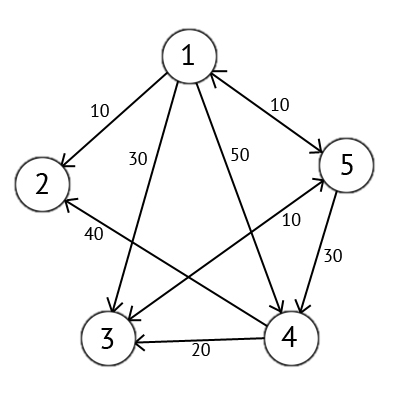
\includegraphics[width=0.4\linewidth]{ad-1.jpg}}
\caption{Пример алгоритма Дейкстры. Исходный граф}
\label{ris:ad-1}
\end{figure}

Возьмем в качестве источника вершину 1. 
Это значит что мы будем искать кратчайшие маршруты из вершины 1 в вершины 2, 3, 4 и 5.
Данный алгоритм пошагово перебирает все вершины графа и назначает им метки, которые являются известным минимальным расстоянием от вершины источника до конкретной вершины. 
Рассмотрим этот алгоритм на примере. 

Присвоим 1-й вершине метку равную 0, потому как эта вершина --- источник. 
Остальным вершинам присвоим метки равные бесконечности (см. рис.~\ref{ris:ad-2}).

\begin{figure}[ht]
\center{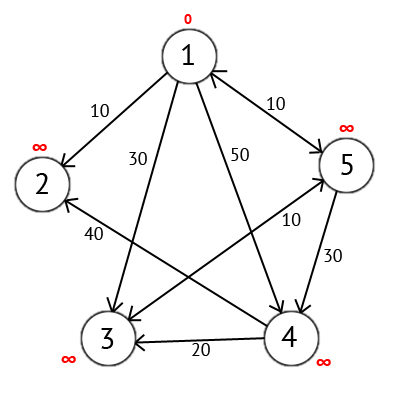
\includegraphics[width=0.4\linewidth]{ad-2.jpg}}
\caption{Пример алгоритма Дейкстры. Инициализация}
\label{ris:ad-2}
\end{figure}

Далее выберем такую вершину $W$, которая имеет минимальную метку (сейчас это вершина 1) и рассмотрим все вершины в которые из вершины $W$ есть путь, не содержащий вершин посредников. 
Каждой из рассмотренных вершин назначим метку равную сумме метки $W$ и длинны пути из $W$ в рассматриваемую вершину, но только в том случае, если полученная сумма будет меньше предыдущего значения метки. 
Если же сумма не будет меньше, то оставляем предыдущую метку без изменений (см. рис.~\ref{ris:ad-3}).

\begin{figure}[ht]
\center{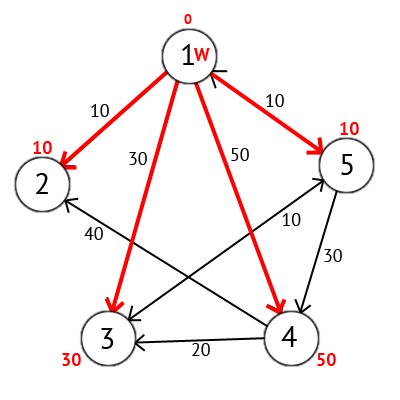
\includegraphics[width=0.4\linewidth]{ad-3.jpg}}
\caption{Пример алгоритма Дейкстры. Первый шаг алгоритма}
\label{ris:ad-3}
\end{figure}

После того как мы рассмотрели все вершины, в которые есть прямой путь из $W$, вершину $W$ мы отмечаем как посещённую, и выбираем из ещё не посещенных такую, которая имеет минимальное значение метки, она и будет следующей вершиной $W$. 
В данном случае это вершина 2 или 5. 
Если есть несколько вершин с одинаковыми метками, то не имеет значения какую из них мы выберем как $W$.

Мы выберем вершину 2. 
Но из нее нет ни одного исходящего пути, поэтому мы сразу отмечаем эту вершину как посещенную и переходим к следующей вершине с минимальной меткой. 
На этот раз только вершина 5 имеет минимальную метку. 
Рассмотрим все вершины в которые есть прямые пути из 5, но которые ещё не помечены как посещенные. 
Снова находим сумму метки вершины $W$ и веса ребра из $W$ в текущую вершину, и если эта сумма будет меньше предыдущей метки, то заменяем значение метки на полученную сумму (см. рис.~\ref{ris:ad-4}).

\begin{figure}[ht]
\center{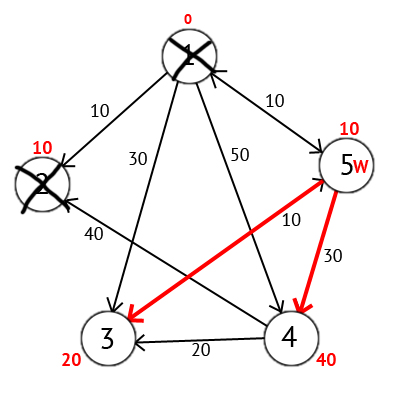
\includegraphics[width=0.4\linewidth]{ad-4.jpg}}
\caption{Пример алгоритма Дейкстры. Второй шаг алгоритма}
\label{ris:ad-4}
\end{figure}

Исходя из картинки мы можем увидеть, что метки 3-ей и 4-ой вершин стали меньше, то есть был найден более короткий маршрут в эти вершины из вершины источника. 
Далее отмечаем 5-ю вершину как посещенную и выбираем следующую вершину, которая имеет минимальную метку.
Повторяем все перечисленные выше действия до тех пор, пока есть непосещенные вершины.

Выполнив все действия получим такой результат (см. рис.~\ref{ris:ad-5})
\begin{figure}[ht]
\center{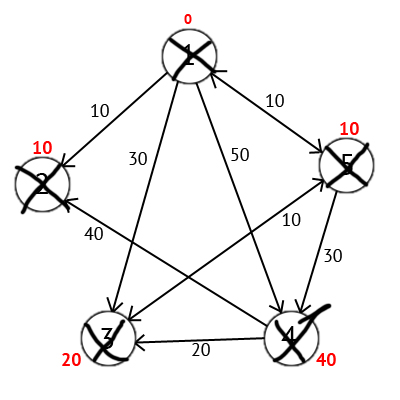
\includegraphics[width=0.4\linewidth]{ad-5.jpg}}
\caption{Пример алгоритма Дейкстры. Конец работы алгоритма}
\label{ris:ad-5}
\end{figure}

Также есть вектор $P$, исходя из которого можно построить кратчайшие маршруты. 
По количеству элементов этот вектор равен количеству вершин в графе.
Каждый элемент содержит последнюю промежуточную вершину на кратчайшем пути между вершиной-источником и конечной вершиной. 
В начале алгоритма все элементы вектора $P$ равны вершине источнику (в нашем случае $P = \{1, 1, 1, 1, 1\}$).
Далее на этапе пересчета значения метки для рассматриваемой вершины, в случае если метка рассматриваемой вершины меняется на меньшую, в массив $P$ мы записываем значение текущей вершины $W$. 
Например: у 3-ей вершины была метка со значением <<30>>, при $W=1$. 
Далее при $W=5$, метка 3-ей вершины изменилась на <<20>>, следовательно, мы запишем значение в вектор $P$ --- $P[3]=5$. 
Также при $W=5$ изменилось значение метки у 4-й вершины (было <<50>>, стало <<40>>), значит нужно присвоить 4-му элементу вектора $P$ значение $W$ --- $P[4]=5$. 
В результате получим вектор $P = \{1, 1, 5, 5, 1\}$. 

Зная что в каждом элементе вектора $P$ записана последняя промежуточная вершина на пути между источником и конечной вершиной, мы можем получить и сам кратчайший маршрут.\cite{ad-habr}

\subsection{Алгоритм А*}
Алгоритм поиска A* --- алгоритм поиска по первому наилучшему совпадению на графе, который находит маршрут с наименьшей стоимостью от одной вершины (начальной) к другой (целевой, конечной).

Порядок обхода вершин определяется эвристической функцией <<расстояние + стоимость>> (обычно обозначаемой как $f(x)$). 
Эта функция --- сумма двух других: функции стоимости достижения рассматриваемой вершины $(x)$ из начальной (обычно обозначается как $g(x)$ и может быть как эвристической, так и нет) и эвристической оценкой расстояния от рассматриваемой вершины к конечной (обозначается как $h(x)$).
Функция $h(x)$ должна быть допустимой эвристической оценкой, то есть не должна переоценивать расстояния к целевой вершине.
Например, для задачи маршрутизации $h(x)$ может представлять собой расстояние до цели по прямой линии, так как это физически наименьшее возможное расстояние между двумя точками.

A* пошагово просматривает все пути, ведущие от начальной вершины в конечную, пока не найдёт минимальный. 
Как и все информированные алгоритмы поиска, он просматривает сначала те маршруты, которые <<кажутся>> ведущими к цели. 
От жадного алгоритма (который тоже является алгоритмом поиска по первому лучшему совпадению) его отличает то, что при выборе вершины он учитывает, помимо прочего, весь пройденный до неё путь (составляющая $g(x)$ --- это стоимость пути от начальной вершины, а не от предыдущей, как в жадном алгоритме). 
В начале работы просматриваются узлы, смежные с начальным; выбирается тот из них, который имеет минимальное значение $f(x)$, после чего этот узел раскрывается. 
На каждом этапе алгоритм оперирует с множеством путей из начальной точки до всех ещё не раскрытых (листовых) вершин графа (<<множеством частных решений>>), которое размещается в очереди с приоритетом. 
Приоритет пути определяется по значению $f(x) = g(x) + h(x)$. 
Алгоритм продолжает свою работу до тех пор, пока значение $f(x)$ целевой вершины не окажется меньшим, чем любое значение в очереди (либо пока всё дерево не будет просмотрено). 
Из множественных решений выбирается решение с наименьшей стоимостью.

Как и алгоритм поиска в ширину, A* является полным в том смысле, что он всегда находит решение, если таковое существует.
Если эвристическая функция $h$ допустима, то есть никогда не переоценивает действительную минимальную стоимость достижения цели, то A* сам является допустимым (или оптимальным), также при условии, что мы не отсекаем пройденные вершины. 
Если же мы это делаем, то для оптимальности алгоритма требуется, чтобы $h(x)$ была ещё и монотонной, или преемственной эвристикой.
Свойство монотонности означает, что если существуют пути $A-B-C$ и $A-C$ (не обязательно через $B$), то оценка стоимости пути от $A$ до $C$ должна быть меньше либо равна сумме оценок путей $A-B$ и $B-C$. 
(Монотонность также известна как неравенство треугольника: одна сторона треугольника не может быть длиннее, чем сумма двух других сторон.) 
Математически, для всех путей $x$, $y$ (где $y$ -- потомок $x$) выполняется:
\begin{equation}
 g(x) + h(x) \le g(y) + h(y).
\end{equation}
A* также оптимально эффективен для заданной эвристики $h$. Это значит, что любой другой алгоритм исследует не меньше узлов, чем A* (за исключением случаев, когда существует несколько частных решений с одинаковой эвристикой, точно соответствующей стоимости оптимального пути).
В то время как A* оптимален для «случайно» заданных графов, нет гарантии, что он сделает свою работу лучше, чем более простые, но и более информированные относительно проблемной области алгоритмы. 
Например, в неком лабиринте может потребоваться сначала идти по направлению от выхода, и только потом повернуть назад. 
В этом случае обследование вначале тех вершин, которые расположены ближе к выходу (по прямой дистанции), будет потерей времени.\cite{AI}

\subsubsection{Пример работы алгоритма А*}


Представим, что у нас есть поле, разделенное на сетку с ячейками, на котором отмечены начальная (зеленая) и конечная (красная) ячейки.
Каждая ячейка имеет состояние (открыта и закрыта), характеризующее её проходимость. 
В примере --- открытые ячейки обведены точками, а закрытые пунктиром.
Принцип алгоритма состоит в том, что он постепенно просматривает все окружающие текущую позицию ячейки и выбирает ячейку с наименьшим «весом».
Стартовая ячейка по умолчанию является первой и единственной «открытой» ячейкой, с которой мы и начинаем поиск пути (см. рис.~\ref{ris:astar-1}).
\begin{figure}[ht]
\center{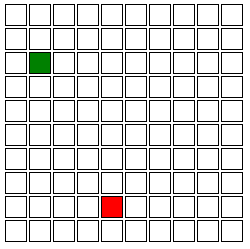
\includegraphics[width=0.4\linewidth]{astar-1.png}}
\caption{Пример алгоритма А*. Исходное поле}
\label{ris:astar-1}
\end{figure}

Теперь мы можем начать поиск пути. 
Ищем у текущей ячейки все «открытые» соседние ячейки и добавляем их в «открытый» список, а текущую ячейку в «закрытый»  (см. рис.~\ref{ris:astar-2}).
\begin{figure}[ht]
\center{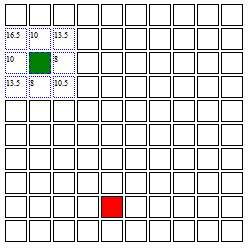
\includegraphics[width=0.4\linewidth]{astart-2.png}}
\caption{Пример алгоритма А*. Первый шаг алгоритма}
\label{ris:astar-2}
\end{figure}

Нужно переместиться в «открытую» соседнюю ячейку, выбрав ту, у которой стоимость ($F$) минимальна.
В нашем примере стоимость ($F$) рассчитывается, как «прямое» расстояние до конечно точки, с учетом того, что ячейки по диагонали имеют вес в 1,5 раза больше, чем ортогональные (не по диагонали). 
Стоимость ячеек для наглядности указана внутри (см. рис.~\ref{ris:astar-3}).
\begin{figure}[ht]
\center{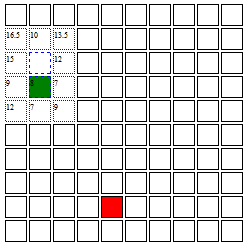
\includegraphics[width=0.4\linewidth]{astart-3.png}}
\caption{Пример алгоритма А*. Второй шаг алгоритма}
\label{ris:astar-3}
\end{figure}

Продолжаем повторение действий:
\begin{itemize}
\item [-] Выставляем текущей ячейке статус «закрытой»;
\item [-] Ищем «открытые» соседние ячейки;
\item [-] Рассчитываем стоимость ($F$);
\item [-] Перемещаемся в ячейку с минимальной стоимостью.
\end{itemize}

В результате мы дойдем до конечной ячейки самым коротким путем (см. рис.~\ref{ris:astar-4}).\cite{astar-habr}
\begin{figure}[ht]
\center{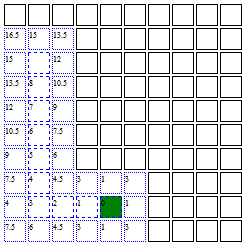
\includegraphics[width=0.4\linewidth]{astart-4.png}}
\caption{Пример алгоритма А*. Конец работы алгоритма}
\label{ris:astar-4}
\end{figure}


\subsection{Волновой алгоритм}

Алгоритм волновой трассировки (волновой алгоритм, алгоритм Ли) --- алгоритм поиска кратчайшего пути на планарном графе. 
Принадлежит к алгоритмам, основанным на методах поиска в ширину.

В основном используется при компьютерной трассировке (разводке) печатных плат, соединительных проводников на поверхности микросхем. 
Другое применение волнового алгоритма --- поиск кратчайшего расстояния на карте в компьютерных стратегических играх.

Волновой алгоритм в контексте поиска пути в лабиринте был предложен Э.Ф.~Муром. 
Ли независимо открыл этот же алгоритм при формализации алгоритмов трассировки печатных плат в 1961 году.

\textbf{Описание алгоритма}.
Алгоритм работает на <<дискретном рабочем поле>> (ДРП), представляющем собой ограниченную замкнутой линией фигуру, не обязательно прямоугольную, разбитую на прямоугольные ячейки, в частном случае --- квадратные. 
Множество всех ячеек ДРП разбивается на подмножества: <<проходимые>> (свободные), т. е при поиске пути их можно проходить, <<непроходимы>> (препятствия), путь через эту ячейку запрещен, стартовая ячейка  (источник) и финишная (приемник). 
Назначение стартовой и финишной ячеек условно, достаточно --- указание пары ячеек, между которыми нужно найти кратчайший путь.

Алгоритм предназначен для поиска кратчайшего пути от стартовой ячейки к конечной ячейке, если это возможно, либо, при отсутствии пути выдать сообщение о непроходимости.

Работа алгоритма включает в себя три этапа: <<инициализацию>>, <<распространение волны>> и <<восстановление пути>>.

Во время инициализации строится образ множества ячеек обрабатываемого поля, каждой ячейке приписываются атрибуты проходимости/непроходимости, запоминаются стартовая и финишная ячейки.

Далее, от стартовой ячейки порождается шаг в соседнюю ячейку, при этом проверяется, проходима ли она, и не принадлежит ли ранее меченной в пути ячейке.

Соседние ячейки принято классифицировать двояко: в смысле окрестности Мура и окрестности фон Неймана, отличающийся тем, что в окрестности фон Неймана соседними ячейками считаются только 4 ячейки по вертикали и горизонтали, в окрестности Мура --- все 8 ячеек, включая диагональные.

При выполнении условий проходимости и непринадлежности её к ранее помеченным в пути ячейкам, в атрибут ячейки записывается число, равное количеству шагов от стартовой ячейки, от стартовой ячейки на первом шаге это будет 1. Каждая ячейка, меченая числом шагов от стартовой ячейки становится стартовой и из неё порождаются очередные шаги в соседние ячейки. 
Очевидно, что при таком переборе будет найден путь от начальной ячейки к конечной, либо очередной шаг из любой порождённой в пути ячейки будет невозможен.

Восстановление кратчайшего пути происходит в обратном направлении: при выборе ячейки от финишной ячейки к стартовой на каждом шаге выбирается ячейка, имеющая атрибут расстояния от стартовой на единицу меньше текущей ячейки. Очевидно, что таким образом находится кратчайший путь между парой заданных ячеек.

Вычислительная сложность волнового алгоритма близка к $O(N^2)$.
В реальных задачах, например при трассировке печатных плат, приложение пути (трассы) выполняется многократно, что влечет существенные временные затраты. \cite{graph-wave}

\subsubsection{Пример работы волнового алгоритма}


ДРП --- это прямоугольник, разбитый на квадратные ячейки одинакового размера. 
Ячейки ДРП подразделяются на свободные, препятствия, источники и приемники. 
На рис.~\ref{ris:wave-1} свободные ячейки имеют светло-зеленый цвет, а препятствия --- светло-коричневый.
Источник залит синим цветом, а приемник --- черным.
Путь может быть проложен только по свободным ячейкам.
\begin{figure}[ht]
\center{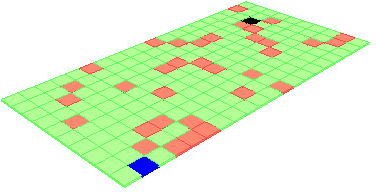
\includegraphics[width=0.4\linewidth]{wv.png}}
\caption{Пример волнового алгоритма. Исходное поле}
\label{ris:wave-1}
\end{figure}

Рассматривается алгоритм построения ортогонального пути. 
Алгоритм состоит из двух частей. 
В первой от источника к приемнику распространяется волна. 
Во второй выполняется обратный ход, в процессе которого из ячеек волны формируется путь.
Волна, идущая от источника к приемнику, на каждом шаге первой части алгоритма пополняется свободными ячейками ДРП, которые, во-первых, еще не принадлежат волне, и, во-вторых, являются 4-соседями ячеек, попавших в волну на предыдущем шаге.
Процесс распространения волны иллюстрируют рис.~\ref{ris:wave-2} -- \ref{ris:wave-5}.

\begin{figure}[ht]
\center{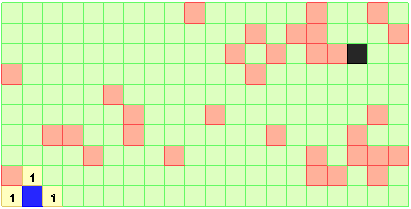
\includegraphics[width=0.4\linewidth]{wv3.png}}
\caption{Пример волнового алгоритма. Первый шаг распространения волны}
\label{ris:wave-2}
\end{figure}

\begin{figure}[ht]
\center{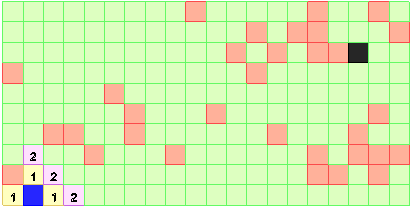
\includegraphics[width=0.4\linewidth]{wv4.png}}
\caption{Пример волнового алгоритма. Второй шаг распространения волны}
\label{ris:wave-3}
\end{figure}

\begin{figure}[h!t]
\center{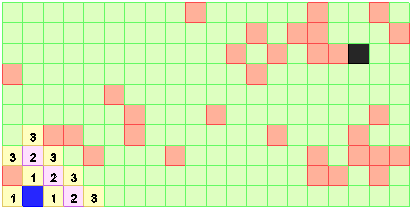
\includegraphics[width=0.4\linewidth]{wv5.png}}
\caption{Пример волнового алгоритма. Третий шаг распространения волны}
\label{ris:wave-4}
\end{figure}

\begin{figure}[h!t]
\center{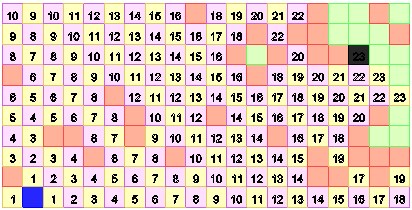
\includegraphics[width=0.4\linewidth]{wv6.png}}
\caption{Пример волнового алгоритма. Последний шаг распространения волны}
\label{ris:wave-5}
\end{figure}

В примере волна достигла ячейку-приемник за 23 шага.
При обратном ходе в путь включается по одной ячейке каждого шага распространения волны. 
При выборе из двух ячеек приоритет имеет ячейка, обеспечивающая горизонтальное продвижение, что приводит к пути, показанному на рис.~\ref{ris:wave-6}.

\begin{figure}[h!t]
\center{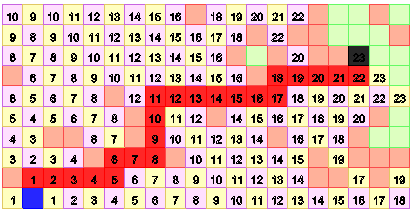
\includegraphics[width=0.4\linewidth]{wv7.png}}
\caption{Пример волнового алгоритма. Обратный ход: формирование пути}
\label{ris:wave-6}
\end{figure}

\section{Сравнительный анализ алгоритмов}
Многообразие алгоритмов поиска пути обусловлено многообразием их применений, для каждого из которых эффективнее работает определенный алгоритм поиска пути.
\begin{itemize}
\item [-] Алгоритм Дейкстры приоритетен в случаях поиска пути до всех точек области поиска, а также в случае отсутствия сколь либо эффективной эвристической функции оценки расстояния между элементами области поиска.
\item [-] Волновой алгоритм эффективен, если область поиска имеет неравномерную проходимость, что затрудняет эвристические вычисления для A*.
\item [-] Алгоритм A* эффективен при одиночном поиске пути между двумя точками, если возможно эффективно эвристически получать примерную дистанцию между элементами области поиска.
\item [-] Навигационная сетка с использованием алгоритма A* эффективна при создании AI, в чьи задачи входит не только поиск пути. Также этот метод эффективен при необходимости построить реалистичную сглаженную траекторию движения между двумя точками. Данный метод предполагает наличие детальной информации об области поиска или возможности получения такой информации.
\item [-] Эвристические алгоритмы поиска пути применимы и оптимальны, если необходим максимально простой алгоритм, при этом область поиска достаточно проста, а применения алгоритма допускают неточность полученного пути.  
\end{itemize}

Таким образом, для построения оптимального порядка планово-профилактического ремонта реактора оптимальным будет использование алгоритма А* к графу ТА-модели реактора.
Особым преимуществом алгоритма А* является наличие эвристической функции.
Это позволяет проводить различные виды оптимизации ППР, изменяя только используемую эвристическую функцию.

\clearpage